\section{Diskrete Fouriertransformation (DFT)}




\subsection{Verwendung}

Die \gls{dft} (Gl. \ref{eq:dft}) ist die zeit- und wertdiskrete Variante der \gls{ft}, die statt von $-\infty$ bis $\infty$ nur von 0 bis N-1 Elemente läuft. 
Im Frequenzspektrum wiederholt sich 
Da es sich um diskrete Werte handelt, geht das Integral in eine endliche Summe über. Die 2D-DFT ist nur möglich (sinnvoll), wenn die Eingangswerte in Form eines Vektors vorliegen.


\subsection{Summen- und Matrizenschreibweise der DFT}
\subsubsection{1D-DFT}
Die \gls{1d-dft} findet wie bereits erwähnt üblicherweise Anwendung, um vom Zeit- in den Frequenzbereich zu gelangen.
\begin{equation}\label{eq:dft}
 X^* \left[ m \right] = \frac{1}{N} \cdot \sum^{N-1}_{n=0} x[n] \cdot e^{-\frac{j 2 \pi m n}{N}}
\end{equation}



Gleichung \ref{eq:1D-DFT_MatrixMult} zeigt die obige Summenformel umgeschrieben zu einer Matrixmultiplikation.

Mit Gleichung \ref{eq:Twiddlefaktorenberechnung} werden zunächst alle Twiddlefaktoren in Matrixform berechnet, wobei n der Index des zu Berechnenden Elements des Vektors im Zeitbereich und
m das Äquivalent im Frequenzbereich ist.
\begin{equation}\label{eq:Twiddlefaktorenberechnung}
\sum^{N-1 }_{m=0} \sum^{N-1 }_{n=0} e^{-\frac{j 2 \pi m n}{N}} = W
\end{equation}


Somit gilt:

\begin{equation}\label{eq:1D-DFT_MatrixMult}
X^* = W \cdot x
\end{equation}

In Matlab kann die Twiddlefaktormatrix mit
\begin{equation}\label{eq:matlab_dft_faktoren}
 W = e^{-\frac{i 2 \pi}{N}\cdot[0:N-1]'\cdot[0:N-1]}
\end{equation}
berechnet werden.


\subsubsection{2D-DFT}
Die \gls{2d-dft} wird hingegen häufig in der Bildverarbeitung verwendet, um vom Orts- in den Fourierraum zu gelagen. Da es sich somit nicht mehr um eine Abhänigkeit 
der Zeit handelt, werden andere Indizes verwendet.
\begin{align}
\begin{split}
X[u,v] 	&= \frac{1}{N} \sum^{N-1}_{n=0} X^* \left[ m \right] \cdot e^{-\frac{j 2 \pi m n}{N}}\\
	&= \frac{1}{MN} \sum^{M-1}_{m=0} \left( \sum^{N-1}_{n=0} f(m,n) \cdot e^{-\frac{j 2 \pi m n}{N}} \right) \cdot e^{-\frac{j 2 \pi m n}{M}}
\end{split}
\end{align}

Auch hier lässt sich die Berechnung in Matrizenschreibweise darstellen:

\begin{align}
\begin{split}
 X &= W \cdot x \cdot W \\
                    &= X^* \cdot W
\end{split}
\end{align}


\subsection{Rein reelle 2D-DFT}
Bei der oben beschriebenen Berechnung können die Eingangssignale auch komplex sein. Da das Ausgangssignal der 1D-DFT unabhängig von den Eingangssignalen in jedem Fall 
komplex ist, kann es dort direkt als Eingangssignal für die komplexe 2D-DFT genutzt werden. 
Es wäre jedoch auch möglich, das komplexe Ausgangssignal der 1D-DFT als zwei von einander unabhängige rein relle Eingangssignale der 2D-DFTs zu betrachten und später 
wieder zusammen zu setzen. 
Diese Umsetzung hat ihren Vorteil darin, dass aus Symmetriegründen die Hälfte der Multiplikationen eingespart werden können. Allerdings ist es erforderlich, dass die 
Hälfte der gespiegelten Werte, nämlich der Imaginärteil, negiert werden muss. Da wie in Abschnitt \ref{sec:Konstantenmultiplizierer} gezeigt wird, die Multiplikation
mit einer Konstanten innerhalb eines Taktes mit einem Schaltnetz erfolgen kann und auch die Negation einen Takt benötigt, ist hier zeitlich kein Gewinn zu erzielen.
Interessant ist dieser Ansatz dann, wenn die Recheneinheit so klein wie irgend möglich gehalten werden soll. Zu bedenken gilt es dann, dass zusätzlicher Speicher für 
Zwischenwerte vorhanden sein muss. Da der Platzbedarf hierfür nicht zu unterschätzen ist, relativiert sich die Ersparnis in gewissem Umfang. Auf eine Gegenüberstellung
wird an dieser Stelle verzichtet, die Berechnung als rein relles Signal wird nachfolgend gezeigt.
Darüber hinaus kann an dieser Stelle bereits gesagt werden, dass aufgrund der zusätzlichen Matrixmultiplikationen mehr Takte für die Berechnung der 2D-DFT benötigt werden.
In Abbildung \ref{pic:reelleDFT} ist die schematische Berechnung der 2D-DFT eines reellen Eingangssignals zu sehen. Hieran lässt sich gut erkennen, dass die Platzersparnis
stark auf kosten der benötigten Zeit ginge. Falls Zeit keine Rolle spielt und Speicher ohnehin vorhanden ist, könnten die zweiten DFTs nacheinander erfolgen.
Um die 2D-DFT eines komplexen Eingangssignals zu berechnen, muss entweder eine identische Einheit für den Imaginärteil vorhanden sein oder noch mehr zeitlich versetzt 
berechnet werden. Die Ergebnisse beider 2D-DFTs müssen identisch zusammengefasst werden, wie es zum Abschluss der einzelnen 2D-DFTs geschechen muss.

\begin{figure}[htbp]
 \centering
 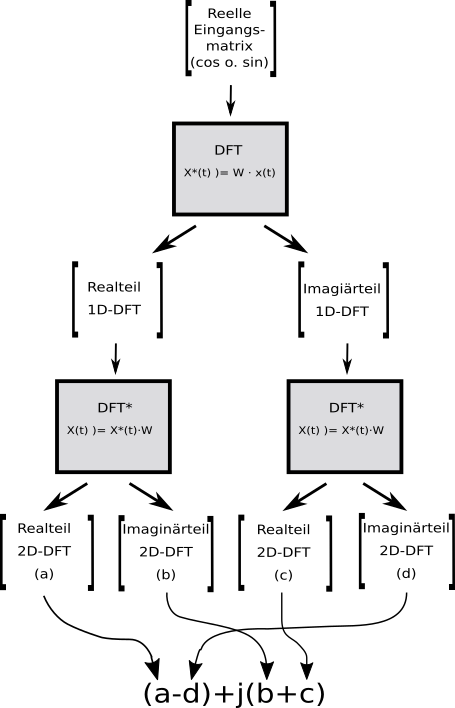
\includegraphics[width=0.5\textwidth]{img/reelleMatMult.png}
 \caption{Veranschaulichung der reellen DFT}
 \label{pic:reelleDFT}
\end{figure}




Da die gegebenen Eingangssignale aus einer Sinus- und einer Kosinuskomponente bestehen und es sich auf diese Weise als ein komplexes Signal auffassen lässt, kann die 
komplexe Berechnung sowohl bei der 1D-DFT als auch bei der 2D-DFT genutzt werden. 
Da hierdurch in beiden Fällen eine vollständige Auslastung einer komplexen Berechnung gegeben ist und wie bereits erwähnt bei der reellen Berechnung zusätzlicher Speicher 
erforderlich wäre, wird dieses Verfahren angewandt.



